\documentclass[12pt]{article}
\usepackage[utf8]{inputenc}
\usepackage[ukrainian]{babel}
\usepackage{amsmath, amssymb}
\usepackage{graphicx}
\usepackage{hyperref}
\usepackage{geometry}
\usepackage{listings}
\geometry{a4paper, margin=2.5cm}

\title{Звіт}



\begin{document}

\section{Вступ}

\texttt{Cancer-cellular-automata} --- це Python-проєкт, що моделює ріст пухлини за допомогою клітинного автомата (КА). Проєкт реалізує дискретну модель, де кожна клітина сітки представляє біологічний стан, що змінюється згідно з локальними правилами.

\section{Структура проєкту}

Основні файли проєкту:

\begin{itemize}
  \item \texttt{cells.py} --- визначає класи клітин та їх стани.
  \item \texttt{grid.py} --- реалізує сітку, де розміщені клітини.
  \item \texttt{visualization.py} --- відповідає за GUI.
  \item \texttt{main.py} --- файл, що запускає програму
  \item \texttt{requirements.txt} --- список залежностей для запуску проєкту.
\end{itemize}

\section{Автомати клітин}
\subsection{Автомат RegularTumorCell (\texttt{RTC})}

Кожна пухлинна клітина є стохастичним скінченним автоматом
\[
\mathcal{A}_{\rm RTC} = \bigl(S_{\rm RTC},\,\Sigma,\,\delta_{\rm RTC},\,s_0^{\rm RTC}\bigr),
\]
де
\begin{itemize}
  \item $S_{\rm RTC} = \{\mathtt{RTC}_k \mid k=0,1,\dots,K\}\cup\{\mathtt{EMPTY}\}$,  
    \begin{itemize}
      \item $\mathtt{RTC}_k$ — клітина з $k$ залишковими діленнями,
      \item $\mathtt{EMPTY}$ — порожня позиція
    \end{itemize}
  \item Вхідний алфавіт 
    \[
      \Sigma = \bigl\{\,\text{мультимножина сусідніх станів}\bigr\}.
    \]
  \item Початковий стан $s_0^{\rm RTC} = \mathtt{RTC}_{K}$.
  \item $s(t)$ - стан автомата на кроці $t$ 
  \item Переходи $\delta_{\rm RTC}(s,\sigma)$ задаються стохастично:
    \begin{enumerate}
      \item {\bfseries Апоптоз:}  
      з ймовірністю $p_{\rm apoptosis}$ - перехіт клітини у порожній стан (її смерть)
      \[
        s(t+1) = EMPTY.
      \]
      \item {\bfseries Розмноження :}  
      якщо $s=\mathtt{RTC}_k$ з $k>0$, з ймовірністю $p_{\rm prolif}$:
      \[
        s(t+1)=\mathtt{RTC}_{k-1},
      \] в сусідній порожній клітинці додається новий автомат в стані $\mathtt{RTC}_{k-1}$.
      \item {\bfseries Міграція:}  
      з ймовірністю $p_{\rm migration}$  
      \[
        s(t+1)=\mathtt{RTC}_k-1,
      \] клітина переходить в сусідню порожню клітинку.
      \item {\bfseries Спокій:}  
      якщо жодна з попередніх подій не сталася,  
      \[
        s(t+1)=\mathtt{RTC}_k-1.
      \]
    \end{enumerate}
\end{itemize}
\begin{figure}[h] % 'h' means 'here', to place the image near this point
    \centering
    \includegraphics[width=0.7\textwidth]{RTC_diagram.png} % Replace with your file name
    \caption{Автомат RTC, k - кількість поділів, що залишились}
    \label{fig:example}
\end{figure}

\subsection{Автомат StemTumorCell (\texttt{STC})}

Стовбурова пухлинна клітина:
\[
\mathcal{A}_{\rm STC} = \bigl(S_{\rm STC},\,\Sigma,\,\delta_{\rm STC},\,s_0^{\rm STC}\bigr),
\]
де
\begin{itemize}
    \item $S_{\rm STC} = \{\mathtt{STC},\,\mathtt{EMPTY}\}$.
    \item Початковий стан $s_0^{\rm STC} = \mathtt{STC}$.
    \item $s(t)$ - стан автомата на кроці $t$ 
    \item Переходи $\delta_{\rm STC}(s,\sigma)$:
    \begin{enumerate}
      \item {\bfseries Апоптоз:}  
      з ймовірністю $p_{\rm apoptosis}$  
      \[
        s(t+1)=\mathtt[{EMPTY}] \text{, в інших випадках стан залишається $STC$}
      \]
      \item {\bfseries Розмноження:}  
      з ймовірністю $p_{\rm prolif}$:
      \[
        \begin{cases}
          &&\text{симетричне ділення (з ймовірністю }p_{\rm symm}\!):\\
            &&\text{$\quad$$\quad$додається новий автомат в стані $\mathtt{STC}$}
            \text{ в сусідню порожню клітинку},\\
          &&\text{асиметричне ділення (з ймовірністю }1-p_{\rm symm}\!):\\
            &&\text{$\quad$$\quad$додається новий автомат в стані $\mathtt{RTC_k}$}
            \text{ в сусідню порожню клітинку}.
        \end{cases}
      \]
      \item {\bfseries Міграція:}  
      з ймовірністю $p_{\rm migration}$ пересувається в порожню сусідню клітинну позицію.
      \item {\bfseries Спокій:}  
      інакше залишається у стані $\mathtt{STC}$.
    \end{enumerate}
\end{itemize}
\begin{figure}[h] % 'h' means 'here', to place the image near this point
    \centering
    \includegraphics[width=0.7\textwidth]{STC_diagram.png} % Replace with your file name
    \caption{Автомат STC}
    \label{fig:example}
\end{figure}
\subsection{Автомат ImmuneCell (\texttt{IC})}

Імунна клітина — більш складний стохастичний автомат:
\[
\mathcal{A}_{\rm IC} = \bigl(S_{\rm IC},\,\Sigma,\,\delta_{\rm IC},\,s_0^{\rm IC}\bigr),
\]
де
\begin{itemize}
  \item $S_{\rm IC} = \{\mathtt{IC}_{L,K} \mid L=0,1,\dots,L_{\max};\, K=0,1,\dots,K_{\max}\}\cup\{\mathtt{EMPTY}\}$,
    \begin{itemize}
        \item $L$ — число вже виконаних успішних атак.
        \item $K$ — поточний вік клітини.
        \item $\mathtt{EMPTY}$ — позиція без клітини.
    \end{itemize}

  \item Початковий стан $s_0^{\rm IC} = \mathtt{IC}_{0}$.
  \item $s(t)$ - стан автомата на кроці $t$ 
  \item Переходи $\delta_{\rm IC}(s,\sigma)$:
    \begin{enumerate}
      \item {\bfseries Апоптоз:}  
      з ймовірністю $p_{\rm apoptosis}$  
      \[
        s(t+1)=\mathtt{EMPTY}.
      \]
      
       \item \textbf{Успішна атака пухлинної клітини:} якщо в сусідах є хоча б одна пухлинна клітина, вибирає ціль і атакує з імовірністю $r_I = \min\Bigl\{1,\ \text{SUCCESS\_RATE}\cdot\frac{n_{\rm IC}}{n_{\rm TC}}\cdot f_{\rm type}\Bigr\}$.
        де:
        \begin{itemize}
        \item $\text{SUCCESS\_RATE}$ — базова ймовірність успішної атаки.
        \item $\frac{n_{\rm IC}}{n_{\rm TC}}$ — відношення кількості імунних клітин ($n_{\rm IC}$) до кількості пухлинних клітин ($n_{\rm TC}$).
        \item $f_{\rm type}$ — кофіціент, що залежить від типу клітини.
      \end{itemize}
       При успіху:
      \begin{itemize}
        \item ціль стає $\mathtt{EMPTY}$.
        \item якщо $L < L_{\max}$, то $s(t) = \mathtt{IC}_{L,K} \to s(t+1) = \mathtt{IC}_{L+1, K+1}$.
        \item якщо $L = L_{\max}$, то $s(t) = \mathtt{IC}_{L_{\max}, K} \to s(t+1) = \mathtt{EMPTY}$.
        \end{itemize}
       \item \textbf{Невдала атака пухлинної клітини:} якщо атака неуспішна, з ймовірністю
      \[
        r_{\rm death} = \min\Bigl\{1,\ \text{DEATH\_RATE} \cdot \frac{n_{\rm TC}}{n_{\rm IC}}\Bigr\}.
      \]
      де:
      \begin{itemize}
        \item $\text{DEATH\_RATE}$ — базова ймовірність загибелі після невдалої атаки.
        \item $\frac{n_{\rm TC}}{n_{\rm IC}}$ — відношення кількості пухлинних клітин ($n_{\rm TC}$) до кількості імунних клітин ($n_{\rm IC}$).
      \end{itemize}
      
      переходить у $\mathtt{EMPTY}$. Тобто, $s(t) = \mathtt{IC}_{L,K} \to s(t+1) = \mathtt{EMPTY}$.
      \item \textbf{Міграція:} з ймовірністю $p_{\rm migration}$
      \[
        s(t) = \mathtt{IC}_{L,K} \to s(t+1) = \mathtt{IC}_{L, K+1}, \quad \text{якщо } K < K_{\max}.
      \]
      де $p_{\rm migration}$ — ймовірність міграції. Міграція відбувається до порожньої сусідньої позиції, що мінімізує відстань до пухлинної клітини. Якщо $K = K_{\max}$, міграція не відбувається.

      \item \textbf{Смерть за віком:} якщо $K = K_{\max}$ (стан $\mathtt{IC}_{L, K_{\max}}$) і не відбувається успішна атака, то
      \[
        s(t) = \mathtt{IC}_{L, K_{\max}} \to s(t+1) = \mathtt{EMPTY}.
      \]
      \item \textbf{Розмноження після вдалого вбивства:} з ймовірністю $p_{\rm prolif\IC}$
      \[
        \text{додається новий автомат } \mathtt{IC}_{0,0} \text{ у порожній сусідній позиції}.
      \]
      де $p_{\rm prolif\IC}$ — ймовірність розмноження. Це відбувається після успішної атаки (перзеходу в стан $\mathtt{IC}_{L+1, K+1}$ або $\mathtt{EMPTY}$ при $L=L_{\max}$).
    \end{enumerate}

\end{itemize}

\begin{figure}[h] % 'h' means 'here', to place the image near this point
    \centering
    \includegraphics[width=0.7\textwidth]{IM_diagram.jpg}
    \caption{Автомат ImmuneCell, k - вік, l - к-сть атак}
    \label{fig:example}
\end{figure}

\section{Лікування}
\label{subsec:chemotherapy}

\subsection{{Хіміотерапія}}
Хіміотерапія в моделі реалізується як зовнішнє втручання, що динамічно змінює параметри пухлинних клітин (\texttt{RegularTumorCell} та \texttt{StemTumorCell}). Основні ефекти:
\begin{itemize}
  \item Зменшення шансу проліферації на фіксований коефіцієнт $\Delta_p = \texttt{PROLIFERATION\_DECREASE}$.
  \item Негайна смерть клітини з шансом $DEATH\_CHEMOTERAPY\_CHANCE}$.
\end{itemize}
Також ракові клітини мають певну стійкіcть до хіміотерапії ($chemotherapy\_resistance$), яка визначається випадково при створенні клітини. Розподіл ймовірності стійкості визначається бета функцією з аргументом $\alpha=0.5$. Після розмноження, нащадки клітини отримують її значення стійкості. Таким чином, з застосуваннями хіміотерапій, на полі буде з'являтись більше клітин, які є менш вразливими до неї.\\

Нехай до застосування хіміотерапії параметри автоматів були:
\[
p_{\rm prolif}^{(0)}.
\]
Після застосування методу \texttt{apply\_chemotherapy()} ймовірність поділу оновлюється так:
\[
    p_{\rm prolif}' &= p_{\rm prolif}^{(0)} + (1 - \Delta_p) \times (1-chemotherapy\_resistance)
\]
Ймовірність негайної смерті під час застосування хіміотерапії визначається як\\
$DEATH\_CHEMOTHERAPY\_CHANCE \times (1-chemotherapy\_resistance)$

\medskip

\subsection{Імунотерапія}
\label{subsec:immunotherapy}

Імунотерапія в моделі посилює функціональні можливості імунних клітин (\texttt{ImmuneCell}). Основні ефекти:
\begin{itemize}
  \item Збільшення максимальної кількості атак: 
    \[
      \mathrm{max\_attacks}' = \mathrm{max\_attacks}^{(0)} + \Delta_a,
    \]
    де $\Delta_a$ — приріст атак (метод \texttt{apply\_immunotherapy()} додає, наприклад, 2 атаки).
  \item Подовження життєвого циклу:
    \[
      \mathrm{lifespan}' = \mathrm{lifespan}^{(0)} + \Delta_\ell,
    \]
    де $\Delta_\ell$ — додаткові кроки життя (наприклад, +10).
  \item Зменшення шансу смерті під час атаки:
    \[
      p_{\rm death}' = p_{\rm death}^{(0)} \times (1 - \Delta_d),
    \]
    де $\Delta_d$ — коефіцієнт зниження (наприклад, 0.2).
  \item Збільшення шансу успішної атаки:
    \[
      p_{\rm success}' = p_{\rm success}^{(0)} \times (1 + \Delta_s),
    \]
    де $\Delta_s$ — приріст ефективності (наприклад, ×3).
\end{itemize}

При виклику методу:


параметри кожної \texttt{ImmuneCell} автоматично оновлюються:
\begin{align*}
  \mathrm{max\_attacks} &\gets \mathrm{max\_attacks} + \Delta_a,\\
  \mathrm{lifespan}     &\gets \mathrm{lifespan} + \Delta_\ell,\\
  \mathrm{death\_chance\_of\_attack} &\gets \mathrm{death\_chance\_of\_attack}\times(1 - \Delta_d),\\
  \mathrm{chance\_of\_succesfull\_attack} &\gets \mathrm{chance\_of\_succesfull\_attack}\times(1 + \Delta_s).
\end{align*}

\medskip


\section{Візуалізація та інтерактивний інтерфейс}
\label{sec:visual-interface}

У \texttt{visualization.py} додано розширений інтерфейс, який дає змогу не лише спостерігати за ростом пухлини, а й управляти симуляцією в реальному часі.

\begin{itemize}
  \item \textbf{Зміна швидкості ітерацій.}  
    Використовується слайдер для налаштування інтервалу між кадрами (у мілісекундах).
  \item \textbf{Відображення статистики.}  
    Над полем виводиться поточна кількість клітин кожного типу: 
    \[
      N_{\rm RTC},\;N_{\rm STC},\;N_{\rm IC}.
    \]
  \item \textbf{Завантаження клітин з файлу.}  
    Кнопка «Load Cells» відкриває JSON-файл (наприклад, \texttt{cells.json}) з попередньо збереженими позиціями й типами клітин.
  \item \textbf{Генерація клітин за допомогою AI.}  
    Кнопка «AI Generate» викликає метод \texttt{ai\_generate\_cells()}, який на основі заданих параметрів (щільності, розміру пухлинного вогнища тощо) створює початковий розподіл клітин.
  \item \textbf{Терапевтичні інструменти.}
    \begin{itemize}
      \item \emph{Chemotherapy:} кнопка застосовує хіміотерапію до всіх пухлинних клітин, автоматично змінюючи коефіцієнти \texttt{PROLIFERATION\_DECREASE} та \texttt{DEATH\_CHEMOTERAPY\_CHANCE}.
      \item \emph{Immunotherapy:} кнопка підсилює імунні клітини викликом методу \texttt{apply\_immunotherapy()}.
    \end{itemize}
  \item \textbf{Налаштування ймовірностей.}  
    Використовується текстове поле (TextBox) для динамічної зміни параметрів кожного типу клітини:
    \[
      p_{\rm apoptosis},\;p_{\rm proliferation},\;p_{\rm migration},\;p_{\rm symm},\;\ldots
    \]
\end{itemize}

\begin{figure}[h] % 'h' means 'here', to place the image near this point
    \centering
    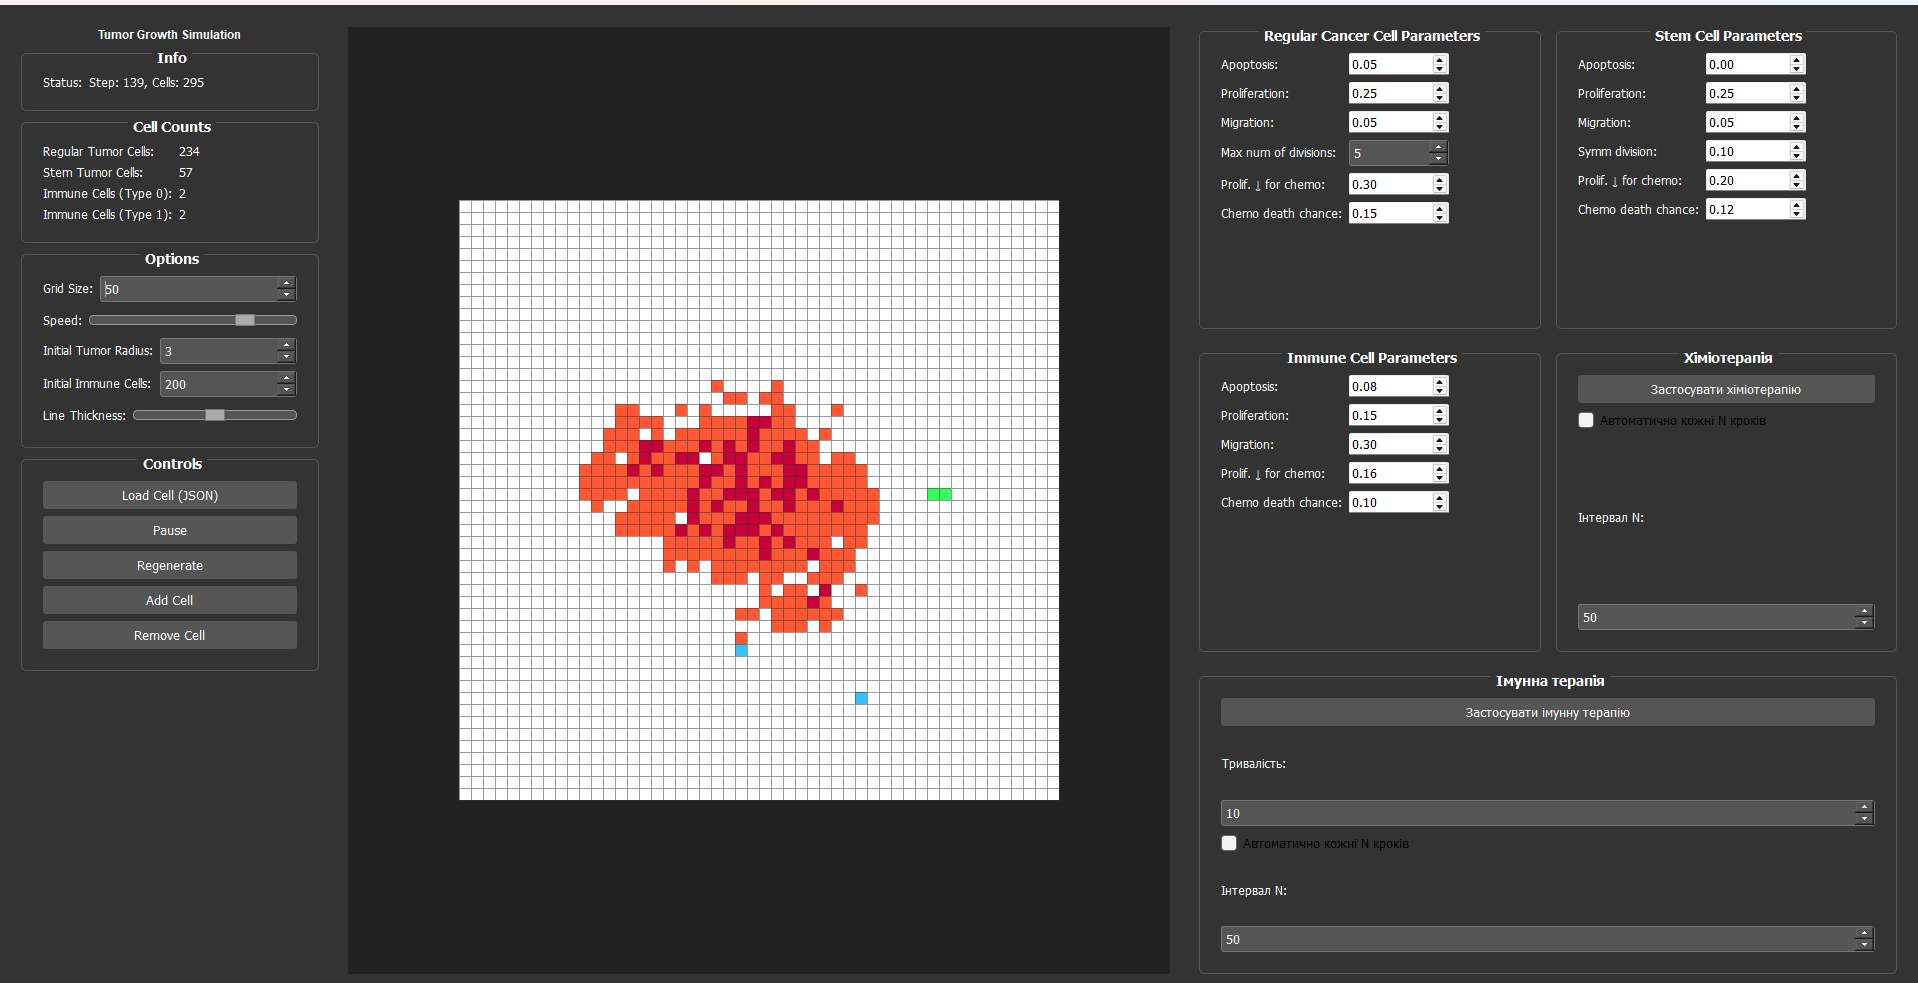
\includegraphics[width=0.9\textwidth]{gui.png} % Replace with your file name
    \caption{Графічний інтерфейс користувача}
    \label{fig:example}
\end{figure}


\section{Завантаження та запуск}

\begin{enumerate}
    \item Клонуйте репозиторій:
    \begin{lstlisting}[language=bash]
git clone https://github.com/your-username/cancer-cellular-automata.git
    \end{lstlisting}
    
    \item Перейдіть в деректорію проєкту:
    \begin{lstlisting}[language=bash]
cd cancer-cellular-automata
    \end{lstlisting}
    
    \item Встановіть залежності:
    \begin{lstlisting}[language=bash]
pip install -r requirements.txt
    \end{lstlisting}
    
    \item Запустіть основну програму:
    \begin{lstlisting}[language=bash]
python main.py
    \end{lstlisting}
\end{enumerate}

\begin{thebibliography}{99}

\bibitem{tumor-growth-dynamics}
Author(s), ``Cellular-automaton model for tumor growth dynamics: Virtualization of different scenarios,''
\url{https://www.sciencedirect.com/science/article/pii/S0010482522011891}

\bibitem{chemotherapy-effects}
Author(s), ``A cellular automata model of chemotherapy effects on tumour growth: targeting cancer and immune cells,''
\url{https://www.tandfonline.com/doi/full/10.1080/13873954.2019.1571515}
\end{thebibliography}

\end{document}
